Note to self: things to keep in mind: research questions and objectives. I want anyone who can read and has a curious mind to understand the introduction and its theme. Unfortunately, I cannot generalize the rest of the thesis beyond someone with a bachelor's degree in math, physics, or engineering. So, for the introduction, I am taking very little for granted when it comes to astronomical knowledge. 

Briefly, in this thesis I pursued the study of stellar streams coming from galactic globular clusters. In essence, these objects are probes of the underlying gravitational field of the Galaxy. Thus, their usecase is an inferrential tool to constrain said gravitational field. However, it is not a simple problem and many aspects need to be explored before the they can be used for their ultimate goal, which is constraining the the galactic distribution of dark matter. My thesis contributes to this aim. But before we can get there, I want to introduce everything from the start. 

For this introduction, I assume the reader is familiar with some basic concepts in astronomy and outer space. To name a few, the heliocentric view of the universe, that gravity is a force of nature, the constant and exponential progression of science and technology from the Renaissance and Enlightenment, that the Earth is round, moon phases, that there are billions of stars within the galaxy, that there are billions of galaxies within the observable universe, that universe is larger than the observable universe, and some basic notions from the big bang theory of cosmology, etc. 

Oftentimes, mes chers compatriotes (people) hold a monolithic and outdated view of astronomy. They envision a romanticized version of the field, where we stay up all hours stargazing with telescopes, switching our gaze back and forth between an eyepiece and a lab notebook. The quickest way to dispel this notion is to draw an analogy to medicine. Everyone understands that many doctors share overlapping knowledge yet specialize in very different areas, resulting in distinct skill sets and daily work routines. 

So when a civilian asks me about my job, I use this analogy by stating that I'm a galactic astronomer. I explain that while I share a common skill set with any physicist, much like a cardiologist shares one with a neurosurgeon, our scope of work can differ drastically.  I inform them that I am interested in explaining the origin and evolution of stars in the galaxy, which is different from, for instance, an astronomer specializing in discovering exoplanets. A neurosurgeon is only responsible for aspects of the human body and biology that pertain to their job. They certainly have a better understanding of the heart than the average person, but not to the same degree as a cardiologist. Likewise, while I may grasp what an astronomer who seeks to discover exoplanets does, I dedicate my time to understanding the galaxy. 

One specific goal in galactic astronomy is understanding dark matter. Before explaining how my research aims to characterize dark matter, I need to set the stage and introduce the cast, tools, and key physical concepts. 


This is a test. 

\begin{figure}
    \centering
    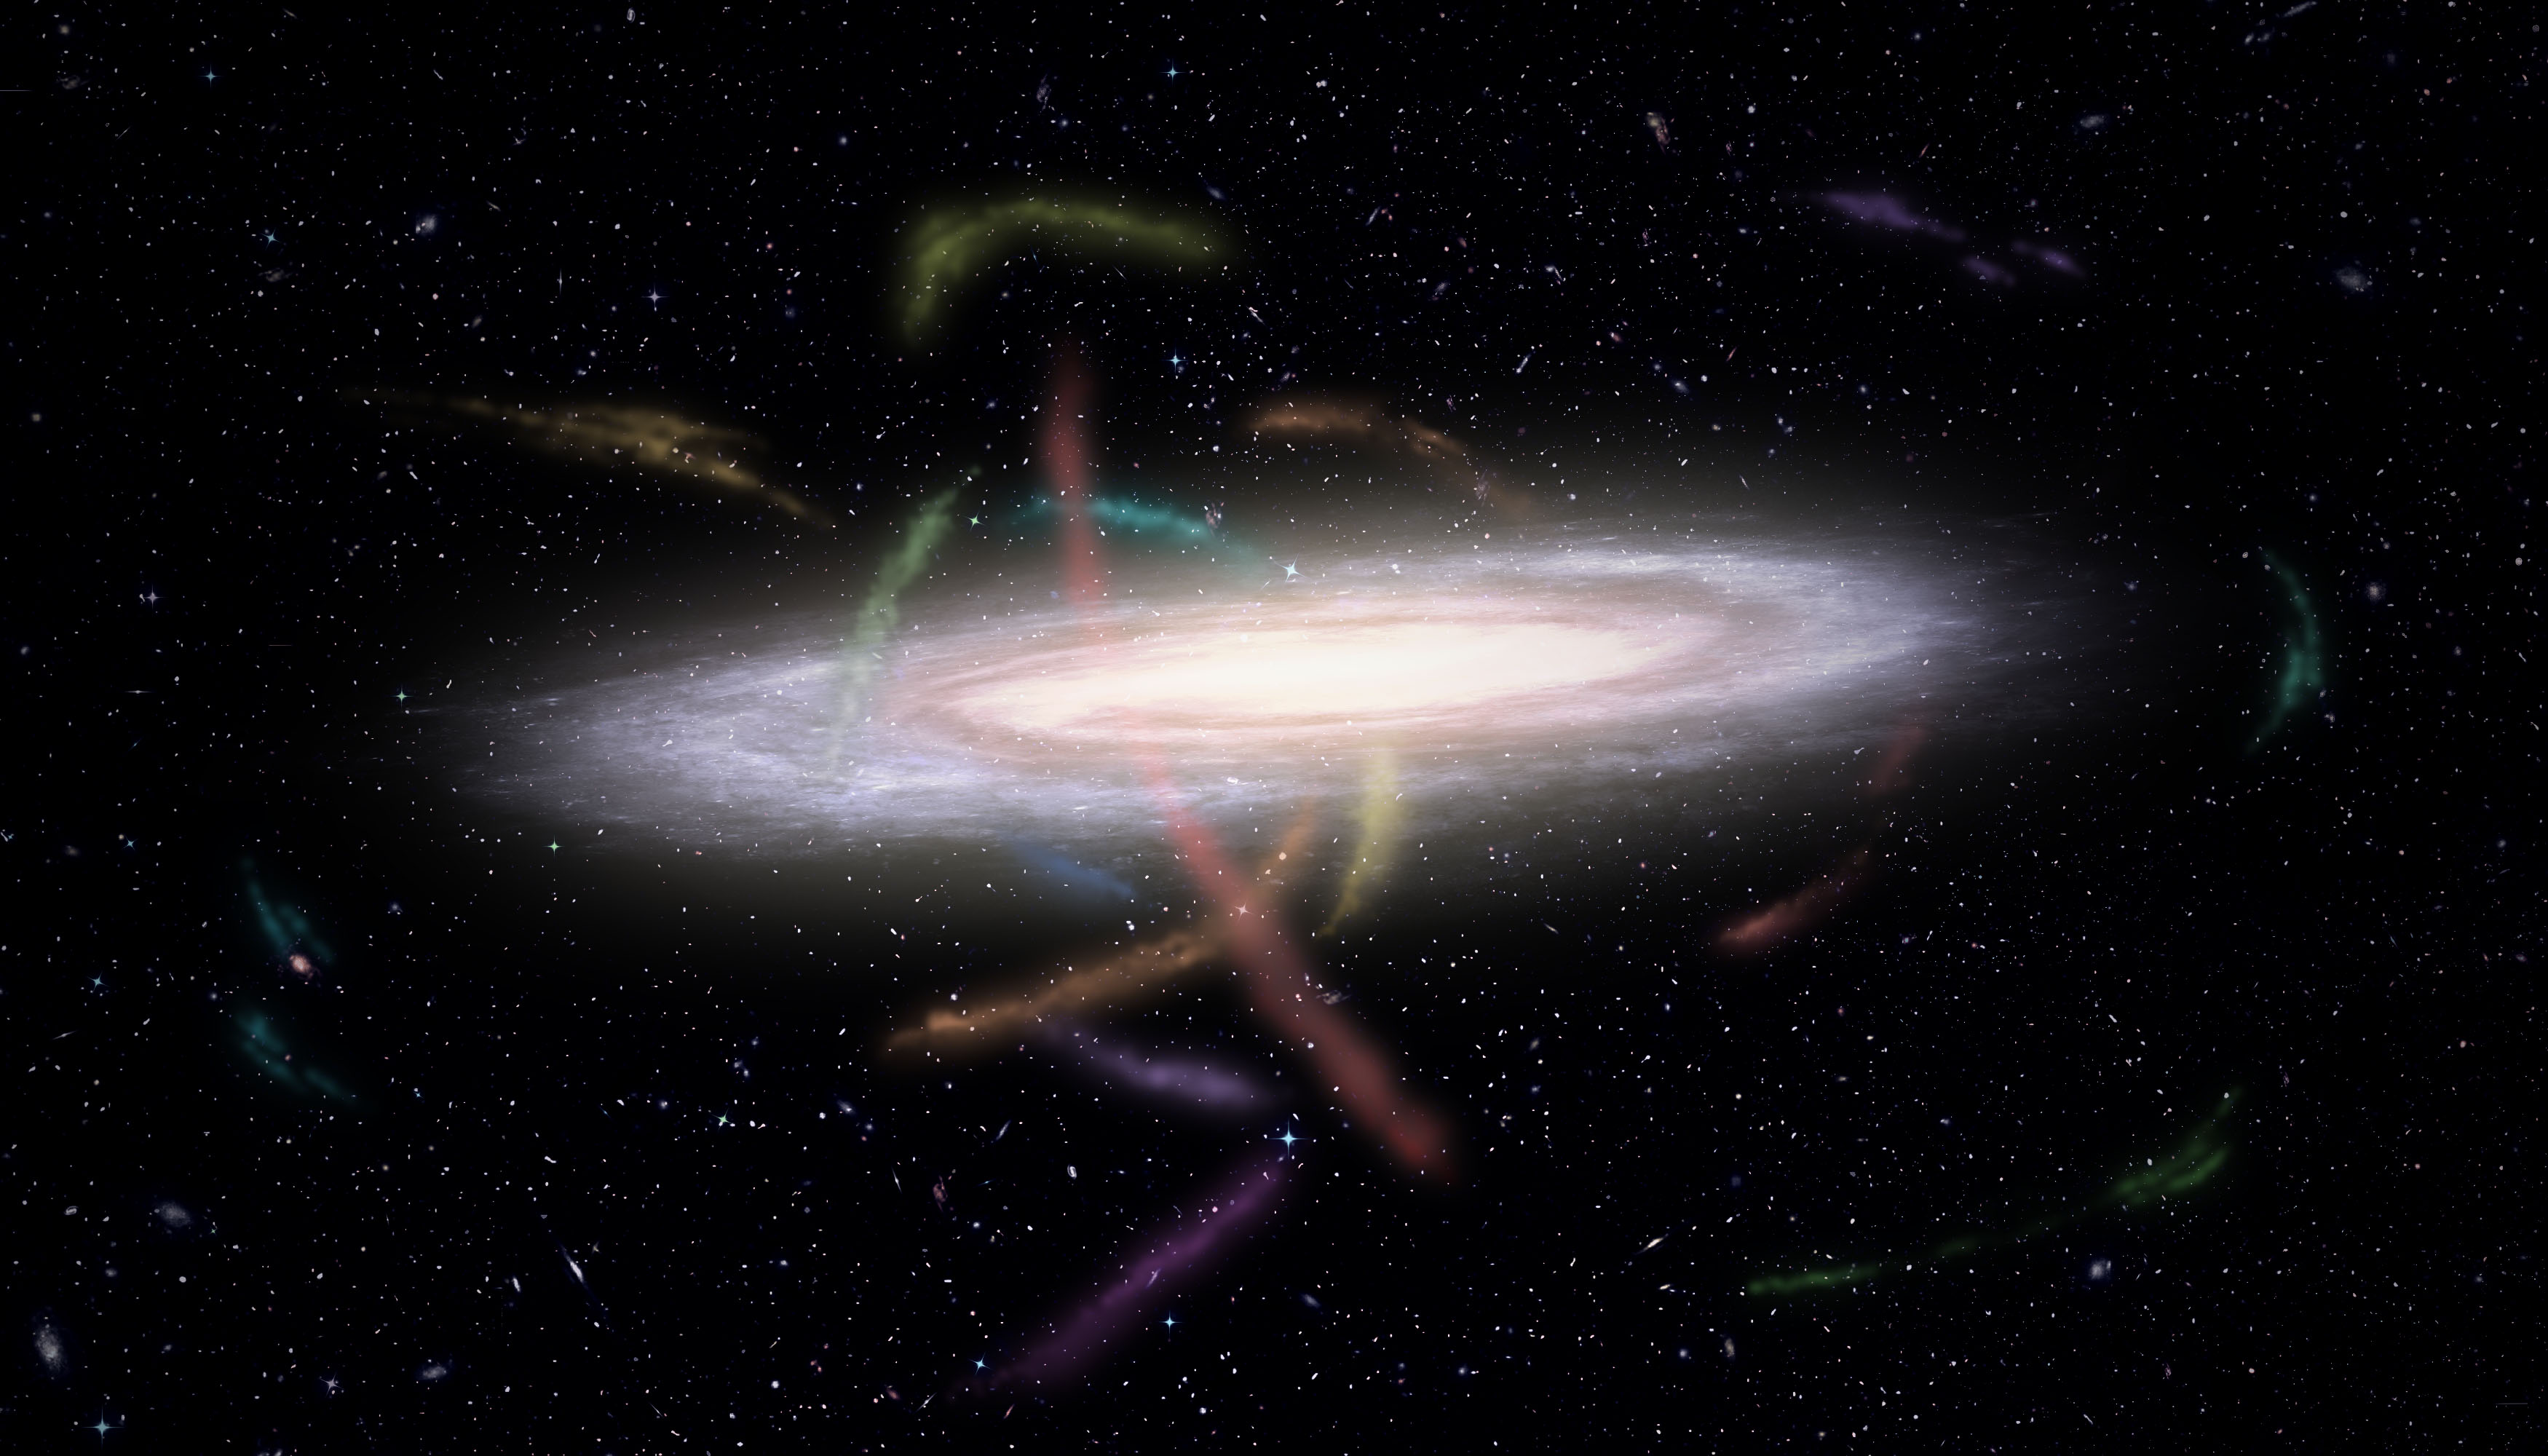
\includegraphics[width=\linewidth]{images/S5MilkywayStreams.jpg}
    \caption{An artist's rendition of a galaxy surrounded by stellar streams. Credit: James Josephides and S$^5$ Collaboration.}
    \label{fig:S5MilkywayStreams}
\end{figure}


\section{The cast: globular clusters and stellar streams}

This cast's two most important characters are stellar streams and globular clusters. Etymology often clarifies scientific terms like nothing else can. Stellar streams are analogous to ordinary streams. Ordinary streams consist of water moving together and pulled by Earth's gravity. On the other hand, stellar streams consist of stars moving together and pulled by a Galaxy's gravity.

Globular clusters belong to a more generalizable group of objects known as star clusters, i.e., groups of stars very close to one another that occupy a small space and are bound together gravitationally. Star clusters exist within galaxies. Globulus is Latin for "spherical" or "globe," hence describing the stars as distributed in a sphere, not in a disk or a box, for example. The two other main types of star clusters are open clusters and nuclear star clusters. The categorical difference between these three is due to differences in their birth, size, and 
location. 

\subsubsection*{Coming from space to teach you about the Pleiades }

Open clusters are the smallest and are named open because they are spread out and not dense. They may have hundreds to thousands of stars within them and are the smallest of the three. A famous open cluster visible in the northern hemisphere is the Pleiades. Within the constellation are about 10 stars visible to the naked eye since they are red giants–the brightest stars, though many more are present. The Pleiades are easily visible as a constellation since the stars group together in a small part of space and have the same color, alluding to their shared origin and similarity. i.e., the stars in an open cluster were born out of the same material and simultaneously. There are many references to the Pleiades from numerous cultures across the world. For example, the ancient Greek writer Homer told us how the sisters instructed them on when to harvest the crops. 

Au lever des filles d'Atlas, des Pléiades, on doit commencer la moisson ; à leur coucher, le labourage. Quarante nuits et quarante jours elles restent cachées, pour ne reparaître que quand l'année a terminé son cours, et qu'on commence à aiguiser les faucilles.

Nuclear star clusters are within the nuclei of galaxies. The fact that their center of mass coincides with the galaxy's center of mass sets them apart from globular and open star clusters. In other words, they are stationary and do not orbit the galaxy. Additionally, globular and open clusters have stars that were born together and from the same clouds of gas. Nuclear clusters have member stars that are not necessarily the same type, but can be diverse. Lastly, galaxies often have supermassive black holes at their centers, which means that we must properly include general relativistic effects when modeling stellar orbits. This distinguishes nuclear star clusters from the others, since the simpler model of gravity, Newtonian mechanics, is insufficient.

\subsubsection*{Hurry Up, We're Dreaming}


\begin{figure}
    \centering
    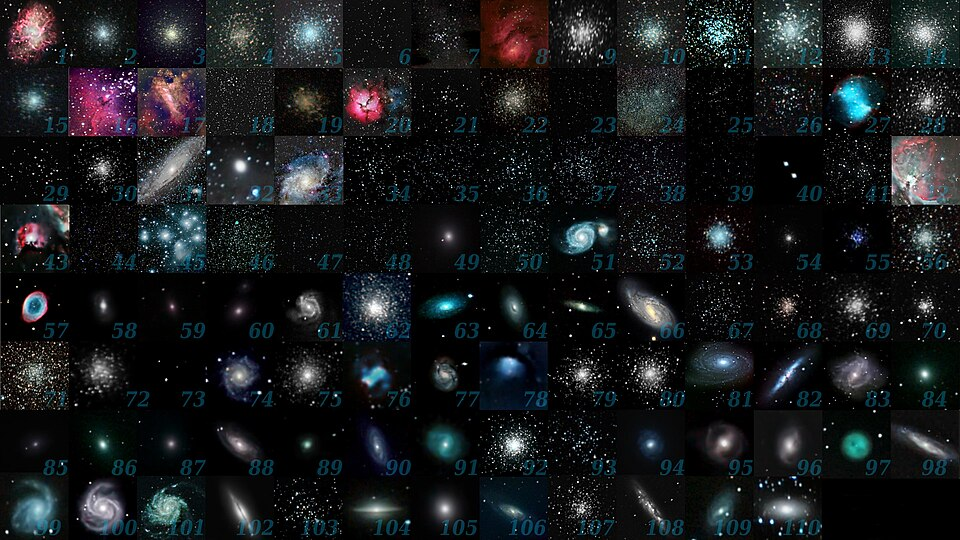
\includegraphics[width=\linewidth]{images/All_messier_objects.jpg}
    \caption{By Michael A. Phillips, an amateur astronomer. - http://astromaphilli14.blogspot.com.br/p/m.html official blog, CC BY 4.0, https://commons.wikimedia.org/w/index.php?curid=38121043}
    \label{fig:All_messier_objects}
\end{figure}



Globular clusters are significantly larger than open clusters, containing thousands to millions of stars and located far from Earth. While a few globular clusters are visible to the naked eye, they appear as a single star due to their distance. Only with a telescope can one distinguish the member stars; indeed, only a powerful telescope can identify the stars individually. For instance, in the 18th century, the technology allowed astronomers to observe that these globular clusters were diffuse, rather than point-like, sources of light, like individual stars. At that time, there was great enthusiasm for discovering transient objects, such as comets. Halley's Comet's next apparition will be in 2061, when I will be 65, which is the typical retirement age in the US. What will the world be like then? Charles Messier created a catalog of non-transient, diffuse objects. In reality, it was a practical dataset intended to save astronomers' time and prevent the rediscovery of the same objects, as well as wasting observation nights in hopes of detecting motion. Only decades later did telescopes become powerful enough to distinguish the stars within globular clusters. Messier's catalog includes nebulae, galaxies, and open and globular clusters. Notably, the spiral galaxy M83 is the namesake of the famous French electronic artist M83, who gained popularity in the 2010s.

Stellar streams are often referred to by many names, frequently using terms like tidal tails or tidal streams–three names for more or less the same thing. Tidal refers to how the stream is created, as opposed to stellar, which pertains to its content. Tidal forces act on extended bodies and cannot affect points. Since gravity's strength diminishes with distance, the central actor has a stronger pull on the near side than the far side. From the center's perspective, the difference in force can rip the body apart. Tidal forces manifest in many ways. On Earth, this appears as water bulging along the line drawn from the moon to Earth's center of mass. NASA provides many fantastic graphics and animations demonstrating the physics of the tides: https://science.nasa.gov/moon/tides/. Tides are also caused by the sun, though they are weaker since the sun is much farther away. Nonetheless, the two tidal forces combine constructively during either a full or new moon, and they combine destructively during the half-moon phase; these are the spring and neap tides, respectively.

Another example within the solar system is Saturn's rings. One proposed formation mechanism is that Saturn's tidal field completely disintegrated a moon body, whose debris was redistributed into a disk. This destruction occurs when the tidal forces exerted by the primary on the secondary are more significant than the secondary's ability to hold itself together gravitationally. Perhaps the most entertaining example, popularized in films and popular science, is the tidal forces from a black hole, as its gravitational force increases rapidly with distance. If a person fell feet-first into the black hole, the gravitational force on their feet would be much stronger than that on their head, causing them to be stretched out or spaghettified. Hence, spaghettification is a tidal phenomenon. 

Stellar streams result from tidal forces disintegrating globular clusters. A moon holds itself together by gravity and electrostatic forces, while the stars in a cluster are bound to one another only by gravity. In practice, tidal forces can either deform or destroy solid bodies. In the case of star clusters, tidal forces may slowly and continuously strip stars from them. This evaporation process produces a steady stream of stars that extends and stretches from the host cluster. We refer to a stream as a tidal tail if it is still attached to a cluster. If a stream is unassociated with a star cluster, the term stellar stream is more appropriate, decoupling it from its inferred origin. However, isn't an iguana's dropped tail still considered a tail?
 


\section{The History of Galactic Astronomy}

If clusters and streams are the characters, the galaxy is the stage. This work focuses on the Milky Way, although other star clusters exist in various galaxies. Rumor has it that some galaxies contain as many as 10,000 globular clusters. Fascinatingly, some studies have observed rogue globular clusters that wander through intergalactic space. While this thesis does not narrate the story of extragalactic astronomy, it remains a valuable reference. 

% First, we inherit the terms "galaxy" and "Milky Way" from ancient Greece, as with much modern science. "Milky Way" is the literal translation of "galaxy," a Greek term. "Gala" (\textgreek{γαλα}) translates to milk, and the suffix "-xy" (-\textgreek{ξίας}) modifies the word into the adjective "milky." Like many ancient civilizations, the Greeks observed the bright expanse of diffuse light in the sky, named it, and associated a mythological story. However, English adopted “Milky Way” through Latin, "Via Lactea," which translates to “Milky Way” or “Milky Path.” In Greek, the original name is "\textgreek{γαλαξίας κύκλος}" (galaxías kýklos), which more accurately translates to "Milky Circle" or "Milky Ring." Thus, the Greeks characterized the structure's shape and position in the sky rather than depicting it as a path to travel on. Referring to a circle aligns with other observations they made about the celestial bodies, such as how the planets all move on the ecliptic — the plane of the solar system where the planets orbit. Of course, the reference to milk would be incredibly evident without light pollution, as on pre-industrial Earth. However, today, we must look up pictures online or travel to remote locations outside major cities to fully grasp the references. Today, a galaxy refers to the general class of massive objects containing billions of stars, while we reserve the name "Milky Way" specifically for our galaxy. 


% Abd al-Rahmān al-Ṣūfī
The story of extragalactic astronomy begins over a thousand years ago, when the Iranian astronomer Abd al-Rahman al-Sufi, in 964 CE, cataloged a faint, blurry patch of light in the sky. In his Book of Fixed Stars, he described what we now call the Andromeda Galaxy as a "little cloud." To him, it was simply a curious smudge, notable but mysterious. For centuries, this “cloud” remained unexplained. When telescopes arrived, observers still didn't know what to make of them. Most wrote it off as a nebula, a fuzzy patch within our Milky Way. It is M31 in Charles Messier's catalog. 

Interestingly, the German philosopher Immanuel Kant published the "Universal Natural History and Theory of the Heavens." In this work, he performed many thought experiments guided by insights from Newton's laws. He was the first to assert that Andromeda, and perhaps other nebulae, were their island universes, similar to our galaxy, each containing an uncountable number of stars, as discussed in the next section.

And then, the idea disappeared. For the next 150 years, the notion of island universes was largely ignored or dismissed. Then, in 1920, there was the now-famous “Great Debate” between Harlow Shapley and Heber Curtis. Shapley argued that the Milky Way was the entire universe, while Curtis revived Kant's hypothesis—that these nebulae were distant galaxies. The truth of the matter was revealed in the years to come. 

It is remarkable to contemplate the concurrent events. Five years prior, in 1915, Albert Einstein published his work on General Relativity, which addresses the fundamental nature of space and time. However, he realized that the equations implied that the universe was either expanding or contracting. The prevailing belief at the time was that the cosmos was eternal and unchanging. Consequently, in 1917, Einstein introduced a term into his equations—the cosmological constant—to account for a static universe.

Look back at history, and astonishingly, Einstein created the equations of general relativity. We recognized the implications of a dynamic and expanding universe before we became aware of other galaxies. A few years later, in 1924, Edwin Hubble studied Cepheid variable stars in the Andromeda “nebula.” He determined their distances, proving that Andromeda exists far beyond the Milky Way. Kant's theory was validated; the universe was unimaginably vast. Hubble broadened his observations, studying the distances of multiple galaxies and measuring their speeds. Five years later, he compiled all these observations and discovered the straightforward linear relationship: the farther you are, the faster you move away from us. The universe is expanding. This relationship is known as Hubble's law.  

I find this rate of change incredible. For 950 years, astronomical conversations involved classifying diffuse celestial objects and debating whether they were nebulae. Then, within just 15 years, we not only established that many galaxies are unimaginably distant from us, but also that the universe is expanding. 

\subsection{Astronomy or astrophysics?}
There is an important point to note in the history of astronomy in this era. I am passionate about etymology and would like to clarify the distinctions between astronomy and astrophysics. I recall when someone inquired if the two were different, and I answered reluctantly and naively, “No, they're just two different names for the same thing." However, a fascinating historical background explains why we use these two separate terms and, as I see it, why they can be considered interchangeable today. 

Astronomy is the oldest science. Before humanity delved into chemistry, biology, or physics, we observed the movements of the stars, with various cultures independently exploring these motions. Until the 1800s, astronomers relied on geometry and mathematics to develop tables that forecasted planetary movements and recorded the positions of stars over time. Essentially, this practice was celestial cartography. It wasn't until the emergence of spectroscopy in the late 1800s that astronomers could investigate stars' chemical and compositional characteristics. In subsequent decades, astrophysics emerged to highlight the application of physics for understanding stellar properties, distinguishing it from the classical study of stellar motions.

Today, making a meaningful contribution to astronomy is virtually impossible without a background in physics, rendering the roles of astronomer and astrophysicist synonymous once again. Astrometry refers to what astronomy once was: the focused study of the positions and movements of celestial bodies. Rather than being a distinct field, it is a necessary component of broader astrophysical studies. 

In some instances, a clear distinction may still be drawn between astrophysicists and astronomers, especially when comparing amateur astronomers to professional scientists. Amateur astronomers harbor a lasting passion for the cosmos. They seek knowledge about constellations and utilize stellar catalogs to engage in astrophotography, often lacking a physics background or professional ambitions. I was surprised the first time I encountered the term “amateur astronomer.” I find it hard to categorize them as amateurs, as this suggests a skill deficiency and feels dismissive. These individuals often possess observational abilities that surpass those of many professional astronomers! While we generally work on computers, only a handful of specific roles entail direct data acquisition and observations. Typically, we wait for data releases from extensive surveys conducted by telescopes on Earth or in space. If we have a particular target in mind, we request telescope time, specifying the necessary instruments, the number of images required, the exposure duration, and the objects to observe. Specialized technicians carry out the observations rather than remote scientists. Many amateur astronomers are more knowledgeable about the night sky than astrophysicists. Moreover, a colleague and former advisor of mine from the Université de la Côte d'Azur has worked with amateur astronomers, tapping into their passion and enlisting their help in dedicated, ongoing observations of the moon! Even today, amateur astronomers play a vital role in scientific exploration. 

\subsubsection*{Kant Rant}
I am compelled to comment further on Kant's \textit{Universal Natural History and Theory of the Heavens}. Reading this work from 270 years ago is truly fascinating. When I first encountered it, I was struck by the fact that Kant authored it—an Enlightenment philosopher I learned about in high school history. I had associated him with figures like Thomas Hobbes and John Locke, rather than with Isaac Newton or Leibniz. What prompts Kant to ponder the solar system's initial conditions? While it's normal for a philosopher to explore cosmic inquiries, the technicality of Kant's questions seems beyond a non-scientist's or non-mathematician's domain. Upon delving into the text, I was even more surprised to find that Kant tackled this issue from a philosophical angle, confirming my initial skepticism. The book contains some arithmetic, yet it lacks equations, graphs, or data tables. 

I find the language use fascinating. I perceive Kant's preface as terse, elitist, and overly complex, with long sentences that introduce multiple ideas at once. I often reread and translate it to grasp the main point. Perhaps his target audience is the societal elite, typical of that time when literacy was scarce.

Furthermore, they assumed that if a writer could manage multiple concepts simultaneously, use a rich vocabulary, and apply various grammatical devices, then he must be intelligent and his ideas must be correct. I can't fault him; he was a product of his era. Here's this excerpt:
This sinking force, which governs throughout the whole space of the planetary system and directs itself to the sun, is thus an accepted natural phenomenon. Equally clearly demonstrated is the law according to which this force extends from the midpoint of the sun into the far distances.
Let us consider this fragment: “equally clearly demonstrated is the law according to which…”... Is that necessary? To understand the text, I translated it as: The sinking force directs planetary bodies toward the sun. This force originates from the sun's center, extends vast distances, and permeates space. Both aspects are accepted laws and natural phenomena. Sometimes, when attempting to understand, I bring a sample of the text to a friend for their interpretation. Amazingly, we are both confounded over the author's true meaning and spend tens of minutes unpacking a single paragraph. In the age of cheap algorithmic content being spoon-fed to us through our mechanical-limb (smart-phones) by the most prominent data companies in the world that employ the best software engineers, and every business and content creator vying for our attention through the most creative and captivating entertainment, we can't be bothered to fight the book just to understand the author. Outrageous. 

I want to highlight how different this is from the writing philosophy I learned. If my writing isn't clear, it indicates a problem–a tragedy. Throughout my education, I've participated in many communication workshops and largely agree with their principles on expressing scientific ideas. This text seems to violate many of those principles. Active voice is crucial, and shorter sentences are preferable, each conveying a single idea. Clarity and brevity are essential; avoid jargon. If I can't understand the text, it suggests the author hasn't fully developed the concept. A text filled with unnecessary jargon may indicate that the author is gatekeeping science, using complex language to appear knowledgeable, or hiding behind complexity to avoid engagement and criticism.

I understand the challenge of effective communication and do not come at authors with my finger on the judgment trigger. I comment on perceptions of authors' values from 200 years ago compared to today. When my writing lacks clarity, it's a disaster, prompting me to reconsider, simplify, or revise the text. Galactic astronomy, mathematics, and computer science are complicated enough.

Furthermore, we are in a new age. Not only are most individuals literate, but they also comprise the public that funds and employs scientists. We work for the public, and our science is our deliverable, making scientific outreach a bonus and a valued asset. Secondly, we are inundated by an abundance of information. If someone struggles to understand my presentation, they will simply move on to something else.

The current zeitgeist differs significantly. Kant was walking a tightrope. In the preface, he goes to great lengths to reassure his religious readers, asserting that his naturalistic account of cosmic formation doesn't threaten faith, but rather celebrates the majesty of creation, that God's greatness lies in having designed a universe so elegant it can run on its own. Unlike Kant, someone explaining the formation of the solar system today does not have to justify themselves. 

Though the tone differs drastically from modern texts, in some places it reads surprisingly familiar. Kant's explanation of linking heaviness to gravity reads incredibly modern. He describes an orbit as free-fall but with enough perpendicular motion to avoid hitting the Earth or the Sun. This explanation is the same that my high school physics teacher, Mr. Calenzo, gave to us. It makes me wonder if we have tended towards the best explanations of physical phenomena independently (if worded in the language of an optimization problem– we all arrived at the “global minimum” in explanation space), or if we are inheritors of these ideas from Kant, in particular. 

Kant's work offers impressive conclusions. He observed that all planets travel in the same direction and plane, even though Newton's laws don't necessitate this arrangement. He acknowledged that no force connects the planets to enforce this configuration. Instead, he concluded that some material must have existed in the past to drive the planets' motions, but is now absent. Remarkably, he reached this conclusion without any knowledge of protoplanetary disks or solar system formation theory. I also found his observations about the “fixed-stars” compelling. First of all, they are just known as stars today. Calling them fixed stars from the modern point of view sounds silly. But at the time, no one had detected their movements. Their stillness made them categorically different from planets and comets. He proposed that perhaps they are not fixed at all, but are instead in motion, with their vast distances making their movement imperceptible. Furthermore, he noted that a large majority of the roughly 2,000 visible stars overlapped with the Milky Way on the sky. This correlation suggested to him that the bright watch patch of the Milky Way was the center of a more extensive system, and that all fixed stars belonged to it, much like planets are bound to the sun.

Essentially, by extending the Copernican Principle —that Earth is not the center of the universe — applying the mediocrity principle, which states that we are typical rather than exceptional, and using the guiding principles of Newtonian mechanics, Kant developed a cosmology and made numerous accurate predictions, even without the supporting data we now have to validate these insights. 

I wonder what Kant would think of the Gaia mission. Not only was he correct in his assertion that the stars are not fixed in place, but we can now detect their motions. Not only can we detect them, but we can detect their motions en masse. Specifically, we have detected the motions of two billion stars, far greater than the 2000 that Kant perceived. Not only is this number vast, but it's only 2\% of the stars in the Milky Way. 

\subsection{The Road to Modern Astornomy}
The introduction of physics into astronomy began in the mid-1800s when Kirchhoff and Gustav applied spectroscopy to the sun and stars, realizing that the bodies in the Heavens are not just magical lights or poked holes in the dark celestial sphere but rather physical objects made of the same materials found on Earth. Since then, people have used physical theories to understand the characteristics of stars and their distribution in the Galaxy. ** insert compelling story about stellar astronomy here ** 

** Insert point about variable stars and standard candles here. Also discuss applying nuclear physics and thermodynamics to understand stellar structure and evolution ** 

From the first half of the 20th century, people continued to apply physics to understand the heavens and improved the quality of their telescopes, building statistics of their observations. For instance, Hubble continued to observe the morphology of galaxies. For many astronomical systems, the time over which something evolves is far longer than a human lifetime. Take, for example, a galaxy. We cannot see the birth and evolution of this object. Still, we can observe hundreds of thousands of galaxies at different stages of life and try to extract general facts about galactic evolution. Similar to looking at the entire human population as it is today. If an alien species were to come to Earth, they might deduce that the tiny ones who are dependent on their parents are younger. Hubble did just this and created what is now known as the Hubble sequence, which is summarized in the schema below. In essence, galaxies are born elliptical, and then preferential rotation flattens them, just like spinning dough. Then, Hubble asserted that there are two possible evolutionary paths. Either the galaxy develops a bar and spiral arms, or develops many spiral arms but no bar. 


\begin{figure}
    \centering
    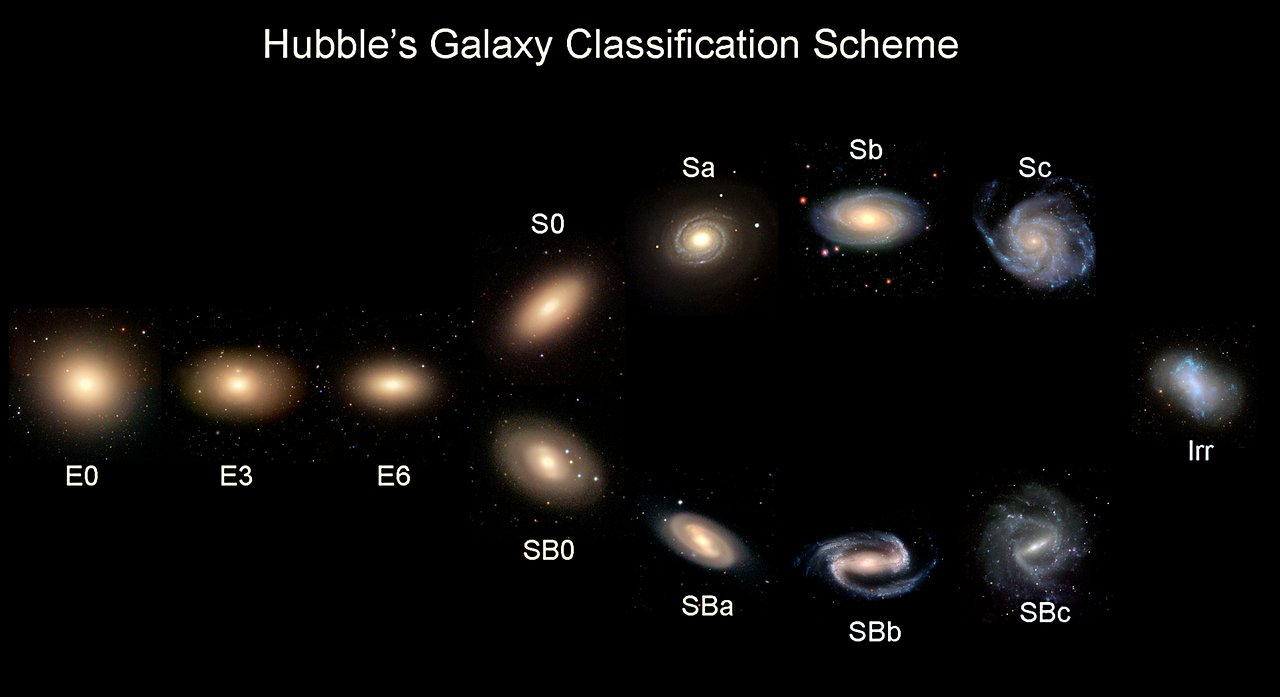
\includegraphics[width=\linewidth]{images/hubble-sequence.jpg}
    \caption{Credit: ESA/Zooniverse}
    \label{fig:Hubble_Tuning_Fork_diagram}
\end{figure}


\subsection{The history of Dark Matter}

Another crucial example is that of Zwicky, a Swiss-American astronomer who investigated a galaxy cluster in the 1930s. A galaxy cluster is a group of galaxies orbiting each other, forming the largest gravitationally bound structures in the universe. The virial theorem explains why a cluster doesn't implode or collapse under its gravity. Essentially, all the bodies must move at certain speeds to avoid infalling and coalescing in the center. If this criterion is met, the bodies will maintain a state of dynamical equilibrium, similar to a pendulum in constant motion. By applying this theorem, Zwicky found that the galaxies were moving much too quickly considering the amount of luminous mass present. A smaller mass suggests that less speed is needed to remain bound to the system since the gravitational pull to the center is weaker. Therefore, the rapid movement of these galaxies indicates the presence of some unseen mass that contributes to the gravitational attraction Zwicky was unable to detect. He coined the term "Dunkle Materie," which is German for "dark matter." 


In terms of setting the groundwork and history of the field leading up to this thesis, the 1930s to 1960s were relatively calm in this regard. From my reads, I am led to believe that it was a period of consolidating the revolution from the aforementioned period in astronomy, as well as advancing the technology. For instance, radio astronomy led to the discovery of the spiral arms within the Milky Way, a feature observed in many other galaxies but previously difficult to detect in our own. 

Specifically, thanks to radio telescopes, astronomers were able to measure the redshift of the H1 21-cm line. From quantum mechanics, this spectral line comes from a ground-state electron transitioning from a parallel to an antiparallel magnetic moment with respect to the proton. Essentially, the difference in energy between these two states is very small, which corresponds directly to a low-frequency photon, or, equally put, a photon with a long wavelength. 

This spectral line is helpful for several reasons. First, since this transition occurs within the centimeter wavelength range, it is transparent to things like dust or gas and can thus travel to the Earth without attenuation. Next, hydrogen is the most abundant element in the universe, which is unsurprising since it is the simplest of all elements. Practically, hydrogen exists in three forms in outer space: ionized hydrogen, atomic hydrogen, or molecular hydrogen. Ionized hydrogen is, of course, just protons. Having it versus atomic hydrogen is a matter of the thermodynamic properties of the medium, where a hotter medium gives more kinetic energy to the electrons and protons, preventing them from bonding. In the case of H2, a catalyst and nucleation site are also needed to facilitate the bonding of two hydrogen atoms. \footnote{Just for fun, singly ionized molecular hydrogen is highly reactive and therefore rare. It is not material used for facilitating astrophysical measurements. Also, for a split second, I considered the conditions for doubly-ionized molecular hydrogen. Upon reflection, I realized that this is silly and only ponder its existence by comparison with double-ionized Helium, which is vital in many astrophysical contexts. This, of course, is a bad comparison since there is no molecular Helium; the two protons in its nucleus are bound through the strong nuclear force. In molecular hydrogen, the two protons are chemically bound together, meaning they share electrons. Without electrons, there can't be any molecular bonds :)}

In any case, atomic hydrogen persists within the interstellar medium, or the space between stars within galaxies. Thus, by measuring the redshift of this line, we can calculate the line-of-sight velocity of the gas. By measuring the line-of-sight velocity around the galaxy, we can create a rotation curve, which measures the circular velocity of the orbital material as a function of distance from the galactic center. 

From any introductory physics course, we know that the speed of an orbit is dictated by the mass of the central attractor. The stronger the gravitational force, the faster you need to go to sustain an orbit and not fall to the center. 

For anyone familiar with this narrative, you know where I'm going with this. In the 1960s, people began measuring the rotation curves of disk galaxies. They noticed that the galaxies were rotating too fast for the amount of mass that could be accounted for by the stars alone. The solution to this problem was to posit the existence of non-luminous matter, which only became mainstream in the late 1970s. However, this wasn't obvious in the 1960s. In fact, during this period, people were still trying to understand the general structure of galaxies. Astronomers were looking to consolidate on the trends set by Hubble and answer the following questions: Why do galaxies have specific surface brightness profiles? What is the best description of how the brightness decreases from the center? Is this relationship independent of the size of the galaxy? Does it depend on the shape of the galaxy? 

Take, for instance, Freeman's work, which was published in 1970. The title of the paper is On the Disks of Spiral and S0 Galaxies. In a nutshell, Freeman begins by discussing the general qualities of elliptical galaxies, which were hitherto better studied than disc galaxies, serving as his motivation for observing and analyzing the galaxies with discs. As per usual, the aim was to study a large sample of galaxies and identify any general trends. Based on this alone, Freeman asserted that the novelty of his work was developing and applying the theory of disc dynamics to interpret a data set of about 30 S0-type galaxies. However, this is not why the paper is cited as much as it is. Indeed, it is most noted for this brief remark made in the appendix about the rotation curve of a specific galaxy: 

The H1 rotation curve has Vmax at R 15', which also happens to be the photometric outer edge of the system. If the H1 rotation curve is correct, then there must be undetected matter beyond the optical extent of NGC 300; its mass must be at least of the same order as the mass of the detected galaxy. There is no optical rotation data for NGC 300.

This brief mention of undetected matter was the first hint towards dark matter since Zwicky's comment in the 1930s. I find it fascinating how science unravels this way, how an afterthought in one paper can become the driving research question in the field. Indeed, in the following years, people continued studying the rotation of galaxies and noticed that their movement was systematically too fast. Initially, as Freeman alluded to, people's initial thought was that the missing matter was just ordinary matter, but unobservable given the wavelength ranges available to them. However, by 1983, Vera Rubin had compiled a literature review in Scientific American and presented all the arguments that ruled out anything but the existence of dark matter. In essence, something else is present that exerts a gravitational force but does not produce any light. Interestingly, Zwicky passed away in 1974. From my readings, I found that he worked in aeronautical engineering for most of the latter half of his career rather than in astronomy. I wonder if he ever found out that his Dunkle Materie became the best fitting explanation. 


** the discovery of the accelerating universe in the 1990s ** 

\subsection{Modern Astronomy}
Since the 1960s and 1970s to today, there have been three additional significant advances that set the stage for today. Firstly, computation. Computers were used in the 1950s, 1960s, and 1970s. However, they were unable to scale to larger problems, which are necessary for astronomy. This was particularly important for cosmology, where you solve a complicated set of PDEs over a large volume… See the works of Navarro Frenk and White… Before this, there was the press-schecter formalism… but in order to obtain an analytical approach to the problem, significant simplifying assumptions needed to be made… Since the 1980s, we have entered an area of running large simulations and then comparing them to observations… 

\subsubsection*{Computational astrophysics}

\subsubsection*{Space based telescopes}

The second revolution is part of the ever-increasing data quality… As space became more accessible, NASA and the European Space Agency began sending telescopes into space to bypass the Earth's atmosphere… Missions like A, B, and C led us to learn X, Y, and Z. 


Lastly, in this current Era of astronomy, we are living in the age of big data, machine learning, Bayesian analysis, and artificial intelligence. High-performance computing facilities have improved like X… Moore's law… 


\subsubsection*{Big data, inference problems, and artificial intelligence }

\section{The Gaia Era}
    \begin{itemize}
        \item This section will be much more techical 
        \item Present some gaia data products 
        \item present the globular cluster catalogue
        \item present eugenes work of the DR3 view of globular clusters 
        \item present Rodrigo's work on detecting the stellar streams 
    \end{itemize}


  Stellar streams are several-kiloparsecs-long structures formed by the tidal disruption of globular clusters or dwarf galaxies orbiting a host galaxy. These tidal forces arise due to differential gravitational pulls across extended objects, causing stars farther from the galactic center to lag behind, while those closer to the center speed up. This stretching creates two tidal tails that trace the cluster's orbit unless in the closest vicinity to the object \citep{2007ApJ...659.1212M}. 
  
  Numerical predictions of this phenomenon have existed since the 1970s \citep[see, e.g.,][]{1975AJ.....80..290K}. These predictions occurred well before the first detections of Galactic globular cluster tidal tails \citep{1995AJ....109.2553G}. Interestingly, \citet{1995AJ....109.2553G}'s detections were made nearly contemporaneously with the discovery of the Sagittarius stellar stream by \citet{1994Natur.370..194I}, which is the closest example of a stream emerging from a dwarf satellite currently interacting with the Milky Way. 
  
  Subsequent studies\footnote{For more subsequent observation detections of tidal debris, i.e., globular cluster stars beyond the tidal radius see the works of: \citet{1997A&A...320..776L, 2000A&A...356..127T, 2000A&A...359..907L, 2001AAS...19910906S, 2003AJ....126..815L,2011ApJ...726...47S,2018MNRAS.476.4814S,2020MNRAS.495.2222S}.} extended Grillmair's findings to other globular cluster streams but were often limited to the detections of stars still close to the cluster tidal radius, until the discovery made by \citet{2001ApJ...548L.165O,2002AAS...200.1001O, 2003AJ....126.2385O} of long and thin tails outside the Palomar~5 globular cluster. With a mass of $1.34\pm 0.24 \times 10^4 M_{\odot}$ \citep{2019MNRAS.482.5138B}, Palomar~5 is one of the least massive globular clusters in the Galaxy. \citet{2003AJ....126.2385O} showed that its tails contain more mass than the cluster. The works of \citet{2006ApJ...641L..37G} and \citet{2015MNRAS.446.3297K} showed that the tails have an extent of more than $20^\circ$ degrees in the sky. The discovery of its prominent tails stimulated a vigorous and successful search in the following years. New streams were discovered, mostly taking advantage of Sloan Digital Sky Survey data, but Pan-STARRS and ATLAS were also used \citep{2006ApJ...643L..17G, 2006ApJ...637L..29B, 2009ApJ...693.1118G, 2012ApJ...760L...6B, 2013ApJ...769L..23G, 2014ApJ...790L..10G, 2015ApJ...812L..26G, 2014MNRAS.443L..84B, 2016MNRAS.463.1759B, 2017ApJ...847..119G, 2014MNRAS.442L..85K}. 
  
  
  \citet{2025NewAR.10001713B} provides a review of stellar stream astronomy, which has entered a new era since the publication of the data from the Gaia astrometric mission \citep{2016A&A...595A...1G}. Gaia's characterization of billions of stars in the Milky Way enables the search for these structures by coupling photometry, astrometry, and spectroscopy for the brightest stars. The possibility given by Gaia to track stars with coherent movements over the entirety of the sky has led to the discovery of dozens of new streams. In addition, \citet{2018MNRAS.477.4063M} developed the \texttt{streamfinder} algorithm and applied it across a series of works \citep{2018MNRAS.481.3442M,  2018ApJ...865...85I, 2019ApJ...872..152I} to discover a multitude of streams.
  
  The possibility of combining Gaia data with spectroscopic surveys has extended the study of stellar streams beyond the quantification of their orbital properties to a full chemical characterization \citep{2019MNRAS.490.3508L, 2020AJ....160..181J, 2021ApJ...911..149L, 2022ApJ...928...30L, 2024MNRAS.529.2413U}. Currently, about a hundred stellar streams are known in our Galaxy. \citet{2023MNRAS.520.5225M} compiled their tracks on the sky into a catalog. Interestingly, only about 20 streams are associated with known Galactic globular clusters.

  One of the interests in studying stellar streams is that they can constrain the gravitational field of their host galaxies, particularly the Milky Way. Compared to the measurement of the HI rotation curve, stellar streams offer the opportunity to investigate the potential of the host galaxy over a wide range of distances, reaching the outermost regions of the halo. For example, \citet{2011MNRAS.417..198V} demonstrated how stellar streams can be used to infer the mass and scale parameters of dark matter halos, utilizing various amounts of observational data, ranging from basic right ascension and declination to full six-dimensional phase space information. \citet{2018ApJ...867..101B} reviewed this concept from an information-theoretic point of view, identifying which orbits and configurations of stellar streams yield the most information about the Galactic potential. However, using single streams to constrain the potential led to ambiguous and non-converging results. For example, \citet{2010ApJ...718.1128L} made use of the Sagittarius stream to infer that the dark matter halo of our Galaxy has a triaxial shape \citep[see also][]{2004MNRAS.351..643H, 2005ApJ...619..800J, 2005ApJ...619..807L}, but \citet{2016ApJ...833...31B} concluded that the dark matter halo of our Galaxy is nearly spherical at the distances of the Palomar~5 and GD-1 streams. The two contrasting results could indicate that the halo is triaxial at one distance but spherical at another, highlighting the need for streams at different distances to map the halo shape. Recently, \citet{2024ApJ...967...89I} constructed a Milky Way model by applying a Markov chain Monte-Carlo (MCMC) fitting procedure. This method identified the set of potential parameters in an axisymmetric model of the Milky Way that best reproduces all observed stellar streams.
  
  
  Beyond the global visible and dark mass distribution streams, streams can also be used to infer the granularity of the dark matter, that is, the mass and density of the subhalos populating our Galaxy. According to simulations by \citet{2008MNRAS.391.1685S}, the $\Lambda$~cold dark matter ($\Lambda$CDM) model predicts that galaxies grow hierarchically, with dark matter clumps forming at a wide range of masses and sizes. These clumps, or subhalos, are predicted to follow a mass distribution with a power-law slope slightly shallower than -2.0. \citet{2012Natur.481..341V} detected the smallest observed dark matter halo through gravitational lensing in an Einstein ring with a mass of $10^8$ solar masses. However, some models predict that dark matter clumps could exist down to at least the mass of Earth-like planets \citep[see]{2005JCAP...08..003G, 2021arXiv211101148A}. 

  \citet{2002MNRAS.332..915I} first suggested that dark matter subhalos could influence stellar streams by diffusing their orbital elements. Later, \citet{2012ApJ...748...20C} expanded this idea, proposing that subhalos could create gaps in stellar streams during flyby encounters, where a subhalo approaches closely enough to a segment of a stream and significantly changes the orbits of the closest stars. \citet{2013ApJ...768..171C} applied this idea and looked for the presence of gaps in the well-known Palomar~5 and GD-1 streams, concluding that the density variations found in their streams were consistent with expectations from $\Lambda$CDM models. \citet{2019ApJ...880...38B} provided further observational evidence for this idea, identifying a gap and a spur in the GD-1 stream that they could not explain by known objects, such as globular clusters, and which they suggested was due to the close passage of a dark matter subhalo. Interestingly enough, as stated in \citet{2019ApJ...880...38B}, the recovered properties of this subhalo (mass and size) were denser than those with the $\Lambda$CDM mass-size relationship presented in \cite{2017MNRAS.466.4974M}. The works mentioned are only a few examples of the extensive literature that has explored the impact of dark matter subhalos in simulated streams \citep{2016ApJ...828L..10H, 2021MNRAS.507.1999H, 2021JCAP...10..043B, 2024arXiv240402953H, 2025ApJ...983...68N} or searched for their traces in observed streams \citep{2016MNRAS.460.2711T, 2017MNRAS.470...60E, 2020ApJ...889...70B, 2020ApJ...892L..37B}.

  In contrast, a limited number of works have explored whether other structures, such as those from baryonic matter, can cause variations in the density of streams and gaps that can be confused with those produced by dark matter subhalos.  Among these works, it is worth mentioning the results of \citet{2017NatAs...1..633P}, which suggest that the presence of the bar at the center of the Galaxy can perturb the characteristics of a stream, such as Palomar~5, and generate gaps along its tail. That the Galactic bar could have an influence on stream morphology was also discussed by \citet{2016MNRAS.460..497H} and \citet{2016ApJ...824..104P}, in the case of the Ophiuchus stream \citep{2014MNRAS.443L..84B}. Besides the Galactic bar, giant molecular clouds can also produce gaps in stellar streams, as shown by \citet{2016MNRAS.463L..17A}. All of these works thus indicate that baryonic structures can play an important role in tail morphology. In this context,  an extensive numerical study specifically focused on modeling the tails of Palomar~5 under the influence of the Galactic bar, spiral arms, giant molecular clouds, and globular clusters, has been realized by \citet{2019MNRAS.484.2009B}, who concluded that both the influence of the bar and that of the giant molecular clouds can leave imprints on Palomar~5 tidal tails similar to those left by dark matter subhalos. In contrast, they found the effect of globular clusters to be negligible. 
  
  Few studies have specifically investigated the effect of globular clusters on stellar streams. \citet{2017MNRAS.470...60E} concluded that globular clusters could not be responsible for the observed density variations in the tails of Palomar~5. Their analysis focused on the characteristics of the observed gaps and involved constraining progenitor properties using reconstructive modeling. By trial and error, they identified a specific configuration of masses, sizes, impact parameters, times of impact, and relative velocities for two perturbers that successfully reproduced the observed density distribution. However, as we do in this work, their method does not perform full forward modeling of the entire globular cluster system on Palomar~5's stream. While they suggest that the impact rate of globular clusters is likely less significant---given their lower abundance compared to the expected dark matter subhalos population---they do not explore this aspect in detail. However, they state that it is an avenue for future investigation. 
  
  More recently, \citet{2022ApJ...941..129D} have examined the possibility that gaps in the GD-1 stellar stream could be due to the close passage of globular clusters, concluding that this scenario is improbable. These first works suggest that the impact of globular clusters on stellar streams is negligible. This result does not necessarily need to be the general case, especially for streams of clusters such as Palomar~5, which live in the inner 20~kpc of the Galaxy, where many other globular clusters also orbit. For example, \citet{2018A&A...620A.154K}, \citet{2019A&A...622A..86M}, and \citet{2023A&A...678A..69I} showed that globular clusters can even collide with other clusters, which implies that cluster stream collisions should happen much more frequently since streams are far more extended than clusters. 
  
  In this study, we aim to fill this gap in the literature on numerically modeling cluster-stream interactions. We seek to quantify the impact of passing globular clusters in the vicinity of streams to understand whether these systems can also be effective and how frequently they alter the distribution of stars in the tails, producing underdense regions or gaps. To this end, in the following pages, we present the results of simulations of the streams of Palomar~5 subject to the gravitational interaction with the set of 165 Galactic globular clusters for which positions and velocities are known to date and for which orbits can therefore be reconstructed \parencite{2021MNRAS.505.5957B}. We chose to simulate streams formed from a cluster with the current characteristics of Palomar~5 because it is a halo cluster with extended tails, and because it is a cluster for which the effect of baryonic structures on its stream has already been studied. As we show, and in tension with previous claims, the close passage of other clusters with such a stream is not rare. Indeed, in the 50 simulations we ran, we found the formation of numerous gaps, averaging 1.5 gaps per simulation, generated by 18 different clusters across the entire system of Galactic globular clusters.


  \subsection{paper1}
Globular clusters are the oldest gravitationally bound stellar systems in the Galaxy \citep{1997A&ARv...8....1M}. About 170 are currently known in the Milky Way \citep{2021MNRAS.505.5978V} and the census is still incomplete, particularly in the inner regions of the bulge and disk of our Galaxy, where  dust extinction and  high stellar number density limit detections. It is in these regions in particular that new globular cluster candidates have been recently discovered, especially thanks to the analysis of near-infrared surveys  
\citep{2011A&A...527A..81M,2011A&A...535A..33M,2017ApJ...838L..14M,2017ApJ...849L..24M,2018ApJ...866...12M,2019A&A...628A..45G,2020A&A...642L..19G,2022A&A...659A.155G,2022A&A...658A.120G,2021A&A...649A..86G,2021A&A...650L..11M,2021A&A...652A.129M,2022MNRAS.509.4962G}.  The current population of globular clusters  is likely to merely represent the leftovers of an initially more numerous and more massive one that had been depopulated as a result of many disruptive processes \citep{1997ApJ...474..223G, 1997MNRAS.288..749M, 1997MNRAS.291..717M, 1997MNRAS.289..898V, fall01}. One of the main processes affecting the globular cluster population and its evolution in number, mass, and size is tidal stripping.   

As all stellar systems are characterized by a finite size and defined orbit of the Galaxy, globular clusters are  subject to tidal effects, which arise because the  opposite sides of these systems experience a different gravitational acceleration. The long-term effect of this process strips the system of its most loosely bound stars, which redistribute themselves onto orbits similar to those of their progenitor, forming so-called ``tidal tails'' or streams around it \citep[see][for some of the earliest studies]{1995AJ....109.2553G, 2000A&A...359..907L}. Some spectacular tails have been discovered and studied  over the past twenty years around Milky Way globular clusters, ranging from the long tails (of roughly $30^\circ$ degrees) departing from the Palomar~5 cluster \citep{2001ApJ...548L.165O, 2003AJ....126.2385O, 2006ApJ...641L..37G, 2009AJ....137.3378O, 2016MNRAS.460.2711T, 2020MNRAS.493.4978S,  2021ApJ...914..123I} to those of NGC~5466 \citep{2006ApJ...637L..29B}, Palomar~14 \citep{2011ApJ...726...47S}, and the GD-1 stream, whose parent cluster has still to be discovered \citep[or has already been completely destroyed, leaving behind the stream as the only vestige of its past existence; see][]{2006ApJ...643L..17G, 2019MNRAS.485.5929W, 2020ApJ...892L..37B}. These studies have been boosted in the last few years thanks to the publication of the ESA Gaia mission catalogues \citep{2016A&A...595A...1G, 2018A&A...616A...1G, 2021A&A...649A...1G, 2021A&A...650C...3G} which has been delivering parallaxes, proper motions, and magnitudes for about 1.4 billion stars, as well as the radial velocities for several million, and thus allowing for searches of stars with coherent distances and motions in the Galaxy, revealing the existence of a number of new and spectacular streams, as well as rediscovering and confirming already known ones \citep[][]{2017ApJ...841L..23N, 2018MNRAS.481.3442M, 2018MNRAS.478.3862M, 2018ApJ...865...85I, 2021MNRAS.505.3033P,  2018ApJ...862..114S, 2019NatAs...3..667I, 2019ApJ...872..152I, 2019MNRAS.484L.114K, bianchini19, 2019ApJ...886L...7M, 2019ApJ...881..106M, 2019MNRAS.488.1535P, 2019MNRAS.485.1029P, caldwell20,  2020ApJ...891..161I, 2020A&A...643A..15P, 2020A&A...637L...2P, 2020A&A...637L...2P, 2020AJ....160..244S, 2016MNRAS.460.2711T, boldrini21, 2021ApJ...914..123I, 2021MNRAS.501..179M, 2021MNRAS.507.1923J, 2021MNRAS.504.2727P, 2021MNRAS.505.3033P, 2021A&A...646A.176P, 2022ApJ...930..103Y, 2022MNRAS.513.3136Z, 2022ApJ...930...23N, 2022MNRAS.509.3709P}. For a general overview, \citet{2023MNRAS.520.5225M} provides a recent compilation of known stellar streams.

All these studies are unraveling  a very complex and rich set of stellar structures in the Milky Way that are mainly distributed in the halo, where their identification is the easiest because of the low density of the background stellar field. 
From a numerical and theoretical point of view, many studies over the years have been focused on the formation and evolution of tidal streams around globular clusters \citep{1975AJ.....80..290K, 1992ApJ...386..506O, 1992ApJ...386..519O, 1998ASPC..136...45G, combes99, 2002MNRAS.332..915I, 2002ApJ...570..656J, 2002JKAS...35...75Y, capuzzo05, 2005CeMDA..91...59D, 2007ApJ...659.1212M, 2008ApJ...681...40S, 2010MNRAS.401..105K, 2010MNRAS.406.2732L, 2012MNRAS.420.2700K, 2012A&A...546L...7M, 2013MNRAS.433.1813S,  2014ApJ...795...95B, 2016MNRAS.463L..17A, 2016MNRAS.463..102E, 2016MNRAS.457.3817S, 2017NatAs...1..633P, carlberg18,  2018A&A...609A..44T, carlberg20, 2022A&A...667A.112V}. These studies have contributed to understanding how these structures form and evolve, to what extent they trace the globular cluster orbit, and how their shape, extension, and morphology depend on the orbital phase and characteristics of the Galactic potential, as well as  on the potential tidal shocks experienced by the cluster itself when it crosses the Galactic disk.


Some works have presented models and simulations for specific streams \citep{2004AJ....127.2753D, 2012A&A...546L...7M, 2019MNRAS.484.2009B, 2019ApJ...880...38B, 2021JCAP...10..043B, 2021DDA....5240106B}, contributing to an understanding of their morphology, density variations, and their extent. From these works, it is clear that the tidal loss of stars from globular clusters and the formation of related structures are important for several reasons: (1) in quantifying to what extent globular clusters have contributed to the field stellar populations, from the halo to the disk to the bulge, and to what extent they still do; (2) reconstructing the properties (in terms of numbers and masses) of the early Galactic globular clusters, through their current mass loss; and (3) using globular cluster streams as a probe of the Galactic potential and, more generally, of the physical laws governing gravity \citep[see, e.g., ][]{2018A&A...609A..44T, bianchini19, 2020PhRvD.102h4066N, 2021JCAP...10..043B}.

In this paper, we wish to contribute to the current discourse on this matter by presenting the first complete catalog of simulated extra-tidal features around globular clusters. We emphasize that we are speaking generically on their features, rather than specifically on tails or streams, because the latter are but one of the morphologies that extra-tidal material can reveal, as we go on to show in this work. This project is motivated, on the one hand, by the aforementioned discoveries of many numerous new streams and  tails in the Galaxy and, on the other hand, by the availability of the full 6D phase information and internal parameters (masses and sizes) for more than 150 Galactic globular clusters \citep{2018MNRAS.478.1520B, 2021MNRAS.505.5957B, 2021MNRAS.501.2279V}. The aims of this project are manifold: (1) to obtain a complete view of the expected distribution of globular clusters tidal structures in the sky; (2) to inform the interpretation of recent and future discoveries; (3) to support the search for new extra-tidal features in the data; (4) to offer the community a repository of all these models to be compared to other theoretical and numerical predictions, which adopt different Galactic potentials and/or gravity laws.    